\documentclass[a4paper,11pt]{article}

\usepackage{times}
\usepackage[T1]{fontenc}
%\usepackage[xetex]{graphicx} % when you compile with xelatex
\usepackage[pdftex]{graphicx} % when you compile with pdflatex
\usepackage{epstopdf}
\usepackage{float}
\usepackage{enumerate}
\usepackage{boxedminipage}
\usepackage{url}
\usepackage{hyperref}
\usepackage{comment}
%\usepackage[dutch]{babel} % when you write in dutch

\usepackage{dcolumn}
\newcolumntype{d}[1]{D{.}{.}{#1}}

%%%%%%%%%%%% layout %%%%%%%%%%%%%%%%%%
\usepackage[margin=3cm]{geometry}
% you might enhance readability by increasing the distances between lines:
%\renewcommand{\baselinestretch}{1.1}

%%%%%%%%%%% mathematics %%%%%%%%%%%%%%%%%%
\usepackage{amsmath,amsfonts,amssymb}

%%%%%%%%%%%%% theorems %%%%%%%%%%%%%%%%
% adapt when you write Dutch

\usepackage{amsthm}

\theoremstyle{plain}
\newtheorem{theorem}{Theorem}
\numberwithin{theorem}{subsection}
\newtheorem{corollary}{Corollary}
\numberwithin{corollary}{subsection}
\newtheorem{proposition}{Proposition}
\numberwithin{proposition}{subsection}
\newtheorem{lemma}{Lemma}
\numberwithin{lemma}{subsection}
\newtheorem{assumption}{Assumption}
\numberwithin{assumption}{subsection}

\theoremstyle{definition}
\newtheorem{definition}{Definition}
\numberwithin{definition}{subsection}
\newtheorem{example}{Example}
\numberwithin{example}{subsection}
\newtheorem{remark}{Remark}
\numberwithin{remark}{subsection}
\newtheorem{notation}{Notation}
\numberwithin{notation}{subsection}

%%%%%%%%%%%%algorithms %%%%%%%%%%%%%%%%%%%
\usepackage{algorithm}
\usepackage{algorithmic}

%%%%%%%%% bibliography style %%%%%%%%%%%%%
\usepackage{natbib} % in case of classic bibtex
%\usepackage[natbib,style=authoryear,maxcitenames=2,
%           maxbibnames=99,hyperref,backend=biber]{biblatex}
%\addbibresource{bib/EORthesis.bib}

%%%%%%%%%%%%%%%% start document %%%%%%%%%%%
\begin{document}

%%%%%%%%%%%%%%% front page %%%%%%%%%%%%%%%%

\thispagestyle{empty}

\includegraphics[height=2cm]{figures/LogoSBE.png}

\vspace*{3cm}

\noindent
\rule{\textwidth}{0.8pt}
\begin{center}
{\huge\bf
\noindent
Deriving fractional moments using the Moment Generating Function
}
\end{center}

\vspace*{-8pt}
\noindent
\rule{\textwidth}{0.8pt}

\vspace*{2cm}

\begin{center}
{\LARGE\bf
Jelle Reisinger
}

{\Large
\vspace*{0.5cm}
(2780350)


\vspace*{2cm}

30 June 2025
}
\end{center}

\vspace*{2cm}

{\Large
\noindent
Bachelor Thesis Econometrics and Data Science
}

\vspace*{1cm}

{\Large
\noindent
Thesis commission:\\[0.3cm]
PhD candidate Gabriele Mingoli\\[0.3cm]
Dr. yyyy (co-reader)
}


\newpage

%%%%%%%%%%%%%%%%%%%%%%% main contents %%%%%%%%%%%%%%%%%
\setcounter{page}{1}

\section*{Abstract}
The abstract should summarize the contents of the thesis.
It should be clear, descriptive, self-explanatory and not longer
than a third of a page. Please avoid using mathematical
formulas as much as possible.
Keywords might be given.

\bigskip\noindent
\textbf{Keywords:} Fractional moments, Moment Generating Function, Fractional Calculus.

\section{Introduction}\label{s:intro}
Statistical moments, defined as the \(n\)-th moment of a random variable \(X\) via its probability density function, are essential tools for characterizing data and its distribution. The first and second order moments, the mean and variance, respectively provide key insights into the average value and dispersion of a random variable. Higher-order moments offer further information about the shape and symmetry of the distribution. A less commonly discussed class of moments, however, are the fractional moments. The latter are defined in precisely the same manner as the integer moments, but now with \(n \in \mathbb{R}\), or even \(n \in \mathbb{C}\). From this point onward, when referring to fractional moments, we denote the order by \(\alpha \in \mathbb{R}\) instead of \(n\). While these moments may not find as much usage in comparison with the integer moments of a distribution, they can be rather valuable in specific applications.
\newline
Fractional moments play a significant role in various fields, including finance, economics, and statistics. One notable application in statistics is their use in approximating integer moments, as described by \cite{inverardi2024}. In such cases, evaluating a 'nearby' existing fractional moment can provide an approximation of the otherwise undefined integer moment \cite{inverardi2024}.
\newline
As an illustration, one can consider the student-t distribution with \(\nu = 2\) degrees of freedom. This distribution only has central and raw moments of order \(k\), where \( 0 < k < \nu\). This implies that its second central moment \((k = 2)\) does not exist. One could however consider the central moment of order \(k\), where \(k = 1.95\), given that this order of the moment does in fact exist and interpret its value as the variance of the distribution. 
\newline
Fractional moments are also used in financial modelling, particularly in the context of Generalized Autoregressive Conditional Heteroskedasticity (GARCH) models. These models are commonly applied to time series data such as financial returns and capture the dynamic volatility that changes over time. The GARCH model achieves this by modelling the volatility based on the returns and variances of previous time periods. It is useful to note that in the context of financial returns, the variable of interest often follows a distribution with heavy tails. As a consequence, not all relevant moments of integer order may exist. In such cases, fractional moments may serve as a viable alternative.  \cite{hansen2024} propose a method for computing fractional absolute moments of the cumulative return, quantities that would otherwise be undefined using traditional integer-order techniques. 
\newline 
In addition, \cite{hansen2024} apply a Heterogenous Autoregressive Gamma Model (HARG) to model intraday stock data. The HARG model assumes the conditional distribution of the variable of interest, say \(X_t\) to be of a non-central Gamma distribution. This model is commonly used to model positive-valued time series data \cite{gourierroux2006}. In particular, the volatility of the random variable is of interest, which by definition is non-negative.
\newline
In this context, \(X_t\) is the realized variance. \cite{hansen2024} study the conditional moments of the variance process. Specifically, they consider moments of order \(\frac{1}{2}, \frac{3}{2}\) and 2 which correspond to the standard deviation, skewness and kurtosis respectively. Furthermore, the moment of order \(-\frac{1}{2}\), the inverse volatility has also been computed. In this context, this moment serves as an estimate of the Sharpe ratio, which is an index to measure the performance of some investment compared to a risk-free asset \cite{sharpe1994}. These fractional moments offer valuable insights into financial return dynamics and are highly relevant for modelling and risk assessment. 
\newline
In a related application, \cite{Mikosc2013} apply fractional moments to financial time series data, focusing on the stationary solution of a stochastic recurrence equation - a recursive formula that describes the evolution of a time series. This equation generalizes common time series models in econometrics such as the ARCH and GARCH and is thus of great interest in the context of financial econometrics. Notably, the GARCH(1,1) model can be represented within this one-dimensional stochastic recurrence equation framework \cite{Mikosc2013}. 
\newline
Similar to the case study by \cite{hansen2024}, conditional moments of fractional order are of great interest, as is often the case in the context of (G)ARCH models. The latter can again be explained by the fact that fractional moments offer a valuable alternative for characterizing the distributional properties of financial time series.
\newline
\cite{gyzl2013} also introduce the use of Fractional moments in risk-models, specifically insurance models. In such models, often the probability density function of total ruin, the event where an insurance company's capital becomes negative, is unknown or difficult to compute. The method of maximum entropy has been developed as a way to approximate these unknown density functions. This method uses fractional moments as input, as they have been proven to be able to characterize its distribution \cite{lin1992}. Compared to traditional techniques, such as inverse Laplace transforms, the maximum entropy approach requires fewer moments to achieve a reliable approximation, making it more computationally efficient and practical for real-world applications. 
\newline
In prior research by \cite{DAmico2002}  the same approach of using fractional moments as input for maximum entropy methods to characterize unknown distributions has been employed. One notable application is in option pricing in A Black-Scholes model. Making use of fractional moments, numerical approximations of theoretical entropies have been obtained. Remarkably, using only two fractional moments, the method achieved approximations with three-digit accuracy.
\newline
 This approach outperformed traditional maximum entropy methods that rely on integer moments, both in terms of accuracy and computational efficiency. Moreover, the use of fractional moments helps to avoid numerical optimization issues that commonly arise when minimizing functions based on integer-moment constraints. Therefore, the results obtained by \cite{DAmico2002} seem to correspond with the aforementioned results obtained by \cite{gyzl2013}. Namely, the implementation of fractional moments in the context of maximum entropy methods has great advantages when it comes to numerical stability and efficiency as compared to more traditional methods. 
\newline
Beyond finance and risk modelling, fractional moments have found valuable applications in fields such as engineering and healthcare. As previously mentioned, \cite{gyzl2024} used fractional moments combined with the maximum entropy method to predict total ruin. This approach has been extended to estimating lifetime distributions, a general topic of interest in survival analysis \cite{clark2003}. Both probability density functions and survival functions were estimated using this technique. Once again, the prediction errors remained within three-digit accuracy, further supporting the method’s consistency and precision across different fields of research.
\newline
Other examples in the field of engineering include optimizing signal processing and control systems as well as studying the response characteristics of random vibration systems. \cite{wang2025} have shown that when using the concept of fractional moments for the latter, accuracy and stability is higher compared to traditional methods, such as Taylor expansions. Furthermore, in terms of simplicity and efficiency, the method of fractional moments is advantageous, as its computation steps are straightforward and avoid convergence issues, significantly reducing the resources required for computation. Implementing the usage of fractional moments has allowed \cite{wang2025} to obtain both analytical, as well as numerical solutions to problems within their research field, which again proves its viability. 
\newline
Another noteworthy application of fractional moments is in the identification of distributions in complex, non-linear systems. \cite{dimatteo2014} demonstrate how complex fractional moments can be used to solve differential equations such as the Kolmogorov or Fokker-Planck equation, which arise in the context of continuous-time Markov processes.
By transforming the system into a more agreeable form using Mellin transforms, \cite{dimatteo2014} show that solutions can be efficiently computed and later recovered using inverse transformations. A key advantage of this method is that it preserves the entire support of the probability distribution, which traditional integer moment methods fail to achieve.
\newline
The remainder of this paper is structured as follows.
Section \ref{s:methodology} discusses existing methods for computing fractional moments, outlining their respective advantages and disadvantages. This section concludes with an introduction to the novel approach proposed in this paper, the required techniques, and the limitations to be mindful of. Section \ref{s:calculus} lays the mathematical foundation for this new method and provides a brief historical overview of the development of fractional derivatives. In section \ref{s: moments}, some key definitions and properties of statistical moments and the moment generating function will be highlighted. What is more, the theory of fractional derivatives from section \ref{s:calculus} will be incorporated in order to extend functionality of the moment generating function. Relevant properties are revisited in this new context, and potential analytical errors of the method are addressed. In section \ref{s:simulation},  simulation results will be analysed, which further clarify the numerical stability and potential errors of computing fractional moments via the moment generating function. Finally, in section 6, the practical implementation of this method in a financial setting will be implemented. The results will be compared against those obtained using traditional methods, with a focus on the implications of potential errors in real-world applications.
\section{Methodology}\label{s:methodology}
\subsection{Existing methods of obtaining fractional moments}
The traditional method of computing fractional moments is rather straightforward. Similarly to integer moments, one simply computes the summation (in the discrete case) or integral (in the continuous case) of \(x^\alpha \cdot f_x(x)\), where \(f_x(x)\) denotes the probability density function of the random variable \(X\). In the context of fractional moments, \(\alpha \in \mathbb{R}\) instead of \(\mathbb{Z}\) (assuming that negative moments exist). \cite{hansen2024} introduce an alternative approach to computing fractional moments using the complex moment generating function (CMGF), which they apply in the context of the aforementioned GARCH models. One of their key expressions is given by:

\[\mathbb{E}\left| X - \xi \right|^\alpha = \frac{\Gamma(\alpha+1)}{2\pi} \int_{-\infty}^{\infty} \frac{e^{-\xi z} M_X(z) + e^{\xi z} M_X(-z)}{z^{\alpha+1}} dt\] \(\text{ where } z = s + it, s \in \mathbb{N_+}, \xi \in \mathbb{R} \) and \(\alpha\) of course the order of the moment.

This formulation extends upon the traditional moment generating function (MGF) but avoids the process of taking derivatives, making it computationally efficient. The inclusion of the Gamma function is logical, as it extends the factorial function to real values, aligning well with the computation of fractional moments. Since this method relies on integration, rather than differentiation, it avoids numerical issues that might arise when computing derivatives, such as obtaining rather great approximation errors.

\subsection{Obtaining fractional moments by using the moment generating function}
While the CMGF method provides an efficient  and elegant alternative to the traditional method, this thesis explores a different approach: computing fractional moments directly by applying fractional derivatives to the MGF. The MGF is widely used for computing integer moments by differentiation around zero. Extending this approach to fractional orders requires us to take fractional derivatives. Thus, we need to define such fractional derivative operators. These fractional derivatives have a long history and often make use of the aforementioned Gamma function in combination with some integral. This means that, for continuous random variables, where we integrate the MGF, we will have to do double integration. A consequence might be that obtaining analytical expressions of these moments may not always be possible. A lot of alternative expressions of these fractional derivatives have been created, mostly based on different interpretations of the latter in the field of physics. In this thesis, we will focus on computing the MGF using the Riemann-Liouville derivative, the Caputo-Fabrizio derivative and the Grünwald-Letnikov fractional derivative. Each of these fractional derivatives in combination with the MGF might lead to different moments expressions for the same distribution and same fractional order of the moment. Thus, it is essential to compare each of these definitions with the traditional way of computing fractional moments, to derive their accuracy and conclude which approach is most suitable for fractional moment computation. Similar to the expression of the moments of a random variable, their 'biases' may also be hard to derive analytically, depending on its distribution.

\subsection{Order and methods of research}
To realize the differences between the aforementioned fractional derivatives, the order of research will be as follows. First, a mathematical groundwork for the fractional derivatives will be laid, in which a number of their respective properties will be discussed. Next, we will revise some basic definitions of statistical moments and the moment generating function and see how some of these properties change when considering fractional moments in combination with the moment generating function. If possible, analytical biases for each fractional derivative in combination with the MGF will be computed, which will conclude the theoretical research of this thesis. We will conduct a simulation using the programming language Julia, to now obtain numerical biases instead of analytical biases. Finally, we will consider a practical case (WIP: TO BE DECIDED) in which all three derivatives will once again be compared.
\section{Fractional Calculus}\label{s:calculus}
In order to obtain the expression as mentioned in section \ref{s:intro}, some advanced tools are required. We can find this in the field of fractional calculus.
We define the following:
\begin{definition}
    Let \(D\) be the differential operator, such that \(D f(x) = \frac{d}{dx} f(x)\). Then the fractional derivative of order \(\alpha\) is defined as \(D^{\alpha} f(x) = \frac{d^{\alpha}}{dx^{\alpha}} f(x)\).
\end{definition}
In this definition, \(\alpha\) can be any real number. When taking regular derivatives, \(\alpha \in \mathbb{N}\). In our case, we are interested in instances where  \(\alpha \in \mathbb{Q_{\geq 0}}\).

It is also possible to study derivatives of negative order, which can be used to obtain moments of negative order of a function. A derivative of negative order is simply an integral of positive order. This is defined as follows:
\begin{definition}
    Let \(J\) be the integral operator, such that \(I f(x) = \int f(x) dx\). Then the fractional integral of order \(\alpha\) is defined as \(I^{\alpha} f(x) = \int f(x) dx^{\alpha}\).
\end{definition}

A lot of different definition have been used to compute a fractional derivative. In this paper, we will focus on the following fractional derivatives:
\begin{definition}
    The Riemann-Louville fractional derivative of order \(\alpha\) is defined as:
    \begin{equation}
        D^{\alpha} f(x) =  \frac{d^{n}}{dx^{n}} D_{x}^{-(n - \alpha)} f(x) = \frac{d^{n}}{dx^{n}} I_{x}^{n - \alpha} f(x) = \frac{1}{\Gamma(\alpha)}  \int_{0}^{x} (x-t)^{\alpha-1} f(t) dt
    \end{equation}
    Where \(n = \lceil \alpha \rceil\), the ceiling function and \(\Gamma(.)\) is the Gamma function, see section \ref{s:appendices}.
   
\end{definition}
A modification of the Riemann-Louville derivative is the Caputo derivative, which is defined as follows:
\begin{definition}
    The Caputo fractional derivative of order \(\alpha\) is defined as:
    \begin{equation}
        D^{\alpha} f(x) = \frac{1}{\Gamma(n-\alpha)}  \int_{0}^{x} (x-t)^{n-\alpha-1} f(t) dt
    \end{equation}
    Where, again \(n = \lceil \alpha \rceil\), the ceiling function and \(\Gamma(.)\) is the Gamma function.
    
\end{definition}

Lastly, we will define the Riesz derivative, which is defined as follows:
\begin{definition}
    The Riesz fractional derivative of order \(\alpha\) is defined as:
    \begin{equation}
        D^{\alpha} f(x) = -\int_{-\infty}^{\infty} |\xi|^{\alpha} \hat{f}(\xi) e^{2\pi i  x \xi} d\xi
    \end{equation}
    Where \(\hat{f}(\xi)\) is the Fourier transform of \(f(x)\).
\end{definition}
%\section{Moments}\label{s: moments}
Having defined the techniques required to compute fractional derivatives, we now turn to their application to the Moment Generating Function (MGF). Before proceeding, we will briefly review some key concepts related to statistical moments.
\subsection{Moments}
\begin{definition}
    Let \(X\) be a random variable.
    The \(\alpha\)-th moment of a \(X\) is defined as:
   \[
\mathbb{E}[X^\alpha] = 
\begin{cases} 
\int_{-\infty}^{\infty} (x - c)^\alpha f_X(x) \, dx & \text{if } X \text{ is continuous,} \\ 
\sum_{i} (x_i - c_ i)^\alpha f_X(x_i) & \text{if } X \text{ is discrete.} 
\end{cases}
\] with, in the context of this paper \(\alpha \in \mathbb{R}\). Here \(f_X(x)\) is the probability density function if \(X\) is a continuous random variable, and the probability mass function if \(X\) is a discrete random variable.
\end{definition}

If \(c = \mu_x\), the first moment of \(f(x)\), then our higher moments are called central moments. In the context of this research, we will focus on the case \(c = 0\), corresponding to raw moments of a random variable \(X\). This choice has been made as the Moment Generating Function, which we will soon define, only computes raw moments of higher order. A moment of order \(n\) is said to exist, if \(\mathbb{E}[X^n] < \infty\).

The following proposition is rather standard and well known. Yet, since we will be working with a lot of fractional moments which replace non-existing integer moments, it does not hurt to reiterate these properties.

\begin{proposition}\label{p: moments_1}
    Let \(X\) be a random variable. Then:
    \begin{enumerate}[(i)]
        \item If \(\mathbb{E}[X^n]\) does not exist, then neither does \(\mathbb{E}[X^k]\), for \( n \leq k\).
    
    \item If \(\mathbb{E}[X^k]\) does exist, then all its lower-order moments, \(\mathbb{E}[X^n]\), for \(n \leq k\). Also exists.
\end{enumerate}
\end{proposition}
The proof is rather straightforward and can be found in Appendix \ref{s:app_B}.


\subsubsection{Moments of negative order}
Since the MGF can be extended to negative orders, we briefly examine how to compute raw moments of negative order using traditional methods. This will allow us to compare results between the two different methods. What is more, as mentioned in section \ref{s:intro}, in specific cases, moments of negative order can be computed to obtain statistics such as the Sharpe Ratio. Thus, it is useful to understand how to compute moments of such orders. We will consider the continuous case:
\[\mathbb{E}[X^{-n}] = \int_{-\infty}^{\infty} x^{-n} f_X(x) dx = \int_{-\infty}^{\infty} \left(\frac{1}{x}\right)^n f_X(x) dx.\] We can immediately observe a rather obvious problem. This integral is undefined at \(x = 0\) and diverges in a neighbourhood around zero. \cite{khuri2002} have stated the following corollary for the existence of a moment with negative first order:
\begin{corollary}
    If \(f_X(x)\) is a continuous pdf defined on \((-\infty, \infty)\), and if \[\lim_{x \to 0} \frac{f_X(x)}{|x|^\alpha} < \infty\] for \(\alpha > 0\), then \[\mathbb{E}[X^{-1}] \text{ exists}.\]
\end{corollary}

Most common distribution functions do not adhere to this corollary, however, the Gamma function does:

\begin{example}\label{e: negative}
    Let \(f_X(x) \sim \Gamma(\alpha, \lambda) =\) 
    \[\frac{x^{\alpha -1} e^{-\lambda x} \lambda^\alpha} {\Gamma(\alpha)}.\] This PDF is defined on \((0, \infty)\). So the function is not defined on \(\mathbb{R}\). This, however, is not a problem, as we can just evaluate the right limit. Since the Gamma function already uses \(\alpha\) as a parameter, we will evaluate \(\frac{f_X(x)}{|x|^\beta}, \beta > 0\):
    \[\lim_{x \to 0_+} \frac{f_X(x)}{|x|^\beta} = \lim_{x \to 0_+} \frac{x^{\alpha -1 - \beta} e^{-\lambda x} \lambda^\alpha} {\Gamma(\alpha)} = \lim_{x \to 0_+} \frac{x^{\alpha -(1 + \beta)} e^{-\lambda x} \lambda^\alpha} {\Gamma(\alpha)} .\] Thus for \(\alpha \geq \beta + 1, \lim_{x \to 0_+} \frac{f_X(x)}{|x|^\beta} < \infty\). Therefore, the first negative moment of the Gamma distribution should exist.

    We will compute the first negative moment: 
    \[ \mathbb{E}[X^{-1}] = \int_{0}^{\infty} x^{-1} \frac{x^{\alpha -1} e^{-\lambda x} \lambda^\alpha} {\Gamma(\alpha)} dx = \frac{\lambda^\alpha}{\Gamma(\alpha)} \int_{0}^{\infty} x^{\alpha - 2} e^{-\lambda x} dx\]
    Using the substitution \( u = \lambda x, \frac{du}{dx} = \lambda, dx = \frac{du}{\lambda}\), we get:
    \[ = \frac{\lambda^\alpha}{\Gamma(\alpha)} \int_{0}^{\infty}\left(\frac{u}{\lambda}\right)^{\alpha -2} e^{-u} du = \frac{\lambda^\alpha}{\Gamma(\alpha) \lambda^{\alpha-1}} \int_{0}^{\infty}(\frac{u}{\lambda})^{\alpha -2} e^{-u} du.\] This integral is equal to \(\Gamma(\alpha - 1)\) (See Appendix \ref{s:appendices}). So we get: 
    \[\mathbb{E}[X^{-1}] = \frac{\lambda^\alpha \Gamma(\alpha - 1) }{\Gamma(\alpha) \lambda^{\alpha-1}} = \frac{\lambda \Gamma(\alpha - 1)}{(\alpha -1)\Gamma(\alpha - 1)} = \frac{\lambda}{(\alpha -1)}.\] Thus, for \(\alpha \neq 1, \mathbb{E}[X^{-1}] = \frac{\lambda}{(\alpha -1)}\). Fortunately, this is always the case, since we had just derived that the integral only converges when \(\alpha \geq \beta + 1, \text{ with } \beta > 0\). In other words, \(\alpha > 1\). So this holds.
\end{example}
\subsection{The Moment Generating Function}
We now formally introduce the Moment Generating Function, one of the most significant subjects of this thesis.
\begin{definition}
    The Moment Generating Function (MGF) of a variable \(X\), is defined as
    \[M_X(t) = \mathbb{E}[e^{tX}]\] provided that \(\mathbb{E}[e^{tX}] < \infty\), for all  \( t \in (- h, h)\), which contains 0, for some \(h > 0\).
\end{definition}

\begin{remark}
    Deriving the expression \(M_X(t) = \mathbb{E}[e^{tX}]\) is typically straightforward. Generally, it simply requires a handful of steps of analytic evaluation. This procedure is not that interesting nor relevant to this research. We provide a single explicit example on how to compute the Moment Generating Function for a specific distribution below. And for later cases, when we make use of an expression of the Moment Generating Function, we will simply refer to the distribution table in Appendix \ref{t: MGF_Appendix}.
\end{remark}

\begin{example}
    Let \(f_X(x) \sim \Gamma(\alpha, \lambda)\) be the Gamma distribution with PDF:
     \[
     f_X(x) = \frac{x^{\alpha -1} e^{-\lambda x} \lambda^\alpha}{\Gamma(\alpha)}.
     \]
     Let \( t < \lambda\) (in any other case, the integral diverges).The moment generating function \(M_X(t)\) is given by:
     \[
     M_X(t) = \int_{0}^{\infty} e^{tx} f_X(x) \, dx = \frac{\lambda^\alpha}{\Gamma(\alpha)} \int_{0}^{\infty} x^{\alpha -1} e^{(t - \lambda) x} \, dx.
     \]
     We make use of the substitution \(u = -(t - \lambda)x\), \(\frac{du}{dx} = (\lambda - t)\), \(dx = \frac{du}{(\lambda - t)}\), so:
     \[
     = \frac{\lambda^\alpha}{\Gamma(\alpha)} \int_{0}^{\infty} \left(\frac{u}{\lambda - t}\right)^{\alpha -1} e^{-u} \frac{du}{\lambda - t} = \frac{\lambda^\alpha}{\Gamma(\alpha) (\lambda - t)^\alpha} \int_{0}^{\infty} u^{\alpha -1} e^{-u} \, du.
     \] This integral is just the definition of the Gamma Function, \(\Gamma(\alpha)\), so we obtain:
     \[ = \frac{\lambda^\alpha \Gamma(\alpha)}{\Gamma(\alpha) (\lambda - t)^\alpha} = \left(\frac{\lambda}{\lambda - t}\right)^\alpha = M_X(t)\]
 \end{example}
 
We will state the theorem which makes the MGF so useful. This theorem allows us to compute moments of higher order by taking derivatives of the given order instead of integrals.
\begin{theorem}\label{t: mgf}
    If \(M_X(t)\) exists on some interval \((-h, h)\), as defined before, we have that:
    \[ \mathbb{E}[X^n] = M_X^{(n)}(0), \text{ for } n \in \mathbb{N}\]
\end{theorem}

\begin{proof}
    The proof is important and fairly straightforward, thus it will be shown directly:
    \[M_X^{(n)}(t) = \frac{d^n}{dt^n} \int_{-\infty}^{\infty} e^{tx} f_X(x) dx = \int_{-\infty}^{\infty} \frac{d^n}{dt^n} e^{tx} f_X(x) dx\] (We can interchange differentiation and integration since all partial derivatives of \(e^{tx} f(x)\) are continuous and the absolute value of the integral converges, as we assume the \(n\)-th moment exists, see Appendix \ref{s:appendices}).
    \[ = \int_{-\infty}^{\infty} x^n e^{tx} f_X(x) dx, \text{evaluating at } t = 0: = \int_{-\infty}^{\infty} x^n e^{0x} f_X(x) dx\]
    \[ = \int_{-\infty}^{\infty} x^n f_X(x) dx = \mathbb{E}[X^n]\]
    The proof for the case that \(f_X(x)\) is discrete is very similar. In that case, one would have to change the order of the derivative and summation, which has also been justified in Appendix \ref{s:appendices}.
\end{proof}


We introduce the following properties for the Moment Generating Function \(M_X(t)\):
\begin{proposition}\label{p: moments}
    For \(X, Y\) random variables, we have that:
    \begin{enumerate}[(i)]
        \item \(M_X^{(0)}(t) = \mathbb{E}[e^{0X}] = 1\). This property can be used to confirm that a given function is a valid probability density function (i.e., integrates to one).
        \item Location scale-transform. Assuming \(M_X(t)\) exists, for constant \(\mu, \sigma\), we have that: 
        \[M_{\mu + \sigma X}(t) = e^{\mu t} \cdot M_X(\sigma t)\]
        \item If \(X \perp Y\), then \(M_{X+Y}(t) = M_X(t)\cdot M_Y(t)\).
    \end{enumerate}
\end{proposition}

The proofs of the latter can be found in Appendix \ref{s:app_B}.

There are several additional topics closely related to the MGF, including Fourier transforms, Laplace transforms, Wick rotations, and characteristic functions. While these subjects are relevant to the theoretical foundation of the MGF , they fall outside the scope of this paper and will therefore not be discussed. Readers interested in exploring these concepts further may find \cite{kolmogorov1999} to be a valuable resource.

\subsubsection{Computing negative moments using the Moment Generating Function}
We have seen that under specific conditions, it is possible to compute negative, or so called inverse moments of distribution functions. This technique can also be applied to the moment generating function. In the 20-th century, \cite{cressie1981} have published the following remarkable theorem:

\begin{theorem}\label{t: negative}
    Assuming the negative \(n\)-th raw moment exists, the negative \(n\)-th raw moment can be computed as follows: 
    \[\mathbb{E}[X^{-n}] = \frac{1}{\Gamma(n)} \int_{0}^{\infty} t^{n- 1} M_X(-t) dt\] where \(n\) is a positive integer.
\end{theorem}
The proof of this Theorem can be found in Appendix \ref{s:app_B}.

Since this is an extension on the regular functions of the MGF, this technique is of interest of this paper. Thus, it will be shortly be discussed. Let us again compute the first inverse moment of the Gamma distribution, but now by making use of the latter theorem for Moment Generating Functions!

\begin{example}
    Let \[f_X(x) \sim \Gamma(\alpha, \lambda) = 
    \frac{x^{\alpha -1} e^{-\lambda x} \lambda^\alpha} {\Gamma(\alpha)}, M_X(t) = \left(\frac{\lambda}{\lambda - t}\right)^\alpha\]
    \[\mathbb{E}[X^{-1}] = \frac{1}{\Gamma(1)} \int_{0}^{\infty} t^{( 1 - 1)} \left(\frac{\lambda}{\lambda - (-t)}\right)^\alpha dt =  \int_{0}^{\infty} \left(\frac{\lambda}{\lambda + t}\right)^\alpha dt\]
    \[ = \lambda^\alpha \int_{0}^{\infty} (\lambda + t)^{-\alpha} dt, \text{ Let } u = \lambda + t, \frac{du}{dt} = 1, dt = du:\]
    \[ \lambda^\alpha \int_{0}^{\infty} u^{-\alpha} du
    =  \lambda^\alpha \frac{u^{ 1-\alpha}}{1 -\alpha}\Big|_{0}^{\infty} = \lambda^\alpha \frac{(\lambda + t)^{1 -\alpha}}{1 -\alpha}\Big|_{0}^{\infty}\]
    \[= \lambda^\alpha\left( 0 - \frac{\lambda^{ 1 - \alpha}}{1 -\alpha}\right) = \frac{-\lambda}{ 1 - \alpha} = \frac{\lambda}{\alpha - 1}.\] Which corresponds with our result from example \ref{e: negative}.
\end{example}

\subsubsection{Extending the MGF to fractional order}
Now that we have introduced the definitions of the MGF and discussed some key properties, we will combine these with the techniques developed in section \ref{s:calculus}. Therefore, we can at last obtain moments of fractional order using the MGF.


To avoid confusion regarding what fractional derivative is being used in combination with the MGF, we will from now on, work with the following notation:
\begin{definition}\label{d: MGF}
    We define the MGF of order \(\alpha \in \mathbb{R}\) by \(\leftindex_{RL}{M}_X^{(\alpha)}, \leftindex_{CF}{M}_X^{(\alpha)}, \leftindex_{GL}{M}_X^{(\alpha)}\) for the MGF in combination with the Riemann-Liouville, Caputo-Fabrizio and Grünwald-Letnikov fractional derivative respectively.
\end{definition}
\begin{remark}
    The three properties mentioned in proposition \ref{p: moments} still hold for the MGF of fractional order. This is the case as the first property makes makes use of the derivative of order 0. Which has been defined to just be the original function itself as stated in the second property of proposition\ref{p: calculus}. The other two properties do not involve any derivatives of any order. Thus, they are generally applicable to the MGF, regardless of its order or kind of derivative.
\end{remark}

Before stating any results about the accuracy of these new MGF expressions, we first consider a numerical example to illustrate the interaction between fractional derivatives and the MGF. 

\begin{example}
    \begin{enumerate}[(i)]
        \item We let \(f_X(x) \sim Bernoulli(p)\), with \(\mathbb{P}(X = 1) = p\) and with associated MGF expression: \(M_X(t) = (1 - p) + p \cdot\exp(t)\), now we consider \[\leftindex_{CF}{M}_X^{(\frac{1}{2})} = \frac{1}{1 - \frac{1}{2}}  \int_{-h}^{t} \exp\left(\frac{\frac{-1}{2}}{1 - \frac{1}{2}}(t-s)\right) f'(s) ds.\] In this case, the domain of \(f(t) = (-\infty, \infty)\), so we let \(-h = -\infty\), and \(f'(s) = p\cdot \exp(s)\), thus we obtain:
        \[\leftindex_{CF}{M}_X^{(\frac{1}{2})} = 2  \int_{-\infty}^{t} \exp\left((s-t)\right) \cdot (p\cdot \exp(s)) ds.\]
        \[= 2p \cdot exp(-t) \int_{-\infty}^{t}\exp(2s) ds\] 
        \[= p\cdot exp(-t) \left(\exp(2s) \Big|_{-\infty}^{t}\right) = p\cdot \exp(t)\]
        Now, all that is left to do is set \(t = 0\) and we obtain that \(\leftindex_{CF}{M}_X^{(\frac{1}{2})} = p\).
        \item Computing \(\mathbb{E}[{X^{\frac{1}{2}}}]\) in the traditional fashion, we obtain: 
        \[\mathbb{E}[{X^{\frac{1}{2}}}] = \sum_x x^{\frac{1}{2}} \mathbb{P}(X = x) = 0^{\frac{1}{2}} \cdot \mathbb{P}(X = 0) + 1^{\frac{1}{2}} \cdot \mathbb{P}(X = 1)\]
        \[ = 0 \cdot(1 - p) + 1 \cdot p = p\]
    \end{enumerate}
    
\end{example}
It is amazing and maybe even somewhat surprising that both expressions obtain the same result. Indeed, this result is actually more of a coincidence. It is important to note that this agreement of results is coincidental and specific to the chosen distribution. Namely, all raw higher moments of a Bernoulli random variable are \(p\). If we had taken any other distribution in combination with a moment of fractional order, it becomes highly likely that the MGF returns a different value compared to the traditional method of computing moments. What is more, if we were to take \[\leftindex_{RL}{M}_X^{(\frac{1}{2})}  = \frac{d}{dt} \frac{1}{\sqrt{\pi}}  \int_{-h}^{t} (t - s)^{\frac{-1}{2}} f(s) ds\] we obtain an integral which may diverge based on the choice of \(-h\) . These observations lead to the following theorem.

\begin{theorem}\label{t: MGF_accurate}
     Consider the three MGF's as defined in definition \ref{d: MGF}. Assume \(\leftindex_{RL}{M}_X^{(\alpha)}\) and \(\leftindex_{GL}{M}_X^{(\alpha)}\) are well defined on some open interval \((-h, h)\), then the moment generating function expressions \(\leftindex_{RL}{M}_X^{(\alpha)}\) and \(\leftindex_{GL}{M}_X^{(\alpha)}\) accurately obtain moments of order \(\alpha \in \mathbb{R}\)
    
\end{theorem}
The proof can be found in Appendix \ref{s:app_B}.
Unfortunately, this result does not hold for \(\leftindex_{CF}{M}_X^{(\alpha)}\), which leads to the following theorem.

\begin{theorem}\label{t: MGF_inaccurate}
    Consider the three MGF's as defined in definition \ref{d: MGF}. Assume \(\leftindex_{CF}{M}_X^{(\alpha)}\) is well defined on some open interval \((-h, h)\), then the moment generating function expression \(\leftindex_{CF}{M}_X^{(\alpha)}\) inaccurately approximates moments of order \(\alpha \in \mathbb{R}\) with approximation error given by
    \[
\begin{cases} 
    \displaystyle \int_{-\infty}^{\infty} x^\alpha  f_X(x) dx -  \displaystyle \int_{-\infty}^{\infty}  \frac{x^{n+1} }{(1 - \beta)x + \beta} f_X(x) dx & \text{if } X \text{ is continuous,} \\ 
    \displaystyle \sum_{i} \left(x_i^\alpha -  \frac{x_i^{n+1} }{(1 - \beta)x_i + \beta}\right) f_X(x_i) & \text{if } X \text{ is discrete.} 
\end{cases}
\] with \(\alpha \in \mathbb{R}, \beta = \alpha - n \text{ and } n = \lfloor \alpha \rfloor.\)
    
\end{theorem}
The proof can be found in Appendix \ref{s:app_B}.

\begin{remark}
    In the case when \(\alpha \in \mathbb{N}\), we have that \(n = \alpha\), and thus \( \beta = 0\), therefore, \(\leftindex_{CF}{M}_X^{(\alpha)}\) is accurate for integer orders. This is an expected result, as the MGF for integer moments is accurate and from section \ref{s:calculus} we know that \(D_{CF}^{\alpha + \beta}f(x) = D_{CF}^\alpha(D_{CF}^\beta f(x))\), with \(\alpha \in \mathbb{N}, \beta \in [0, 1).\) In this case, let \(\beta = 0\). So we get \(D_{CF}^{\alpha + 0}f(x) = D_{CF}^{\alpha}f(x)\) which is just a regular derivative of integer order.
\end{remark}
\subsubsection{Analysing the error of the Caputo-Fabrizio MGF}
We now further inspect the error obtained in theorem \ref{t: MGF_inaccurate}. Note that in the following plots, we explicitly focus on the term \[ E(x, \alpha) = x^\alpha - \displaystyle \frac{x^{n+1} }{(1 - \beta)x + \beta}\] for simplicity. The expression we analyse, denoted \(E(x, \alpha)\) is not the same as the expression obtained in theorem\ref{t: MGF_inaccurate}. Yet, it is the part of the expression that involves the order \(\alpha\) and is thus of great interest. What is more, considering the result obtained in theorem \ref{t: MGF_inaccurate}, it is easy to see that \(\leftindex_{CF}{M}_X^{(\alpha)}\) is accurate \(\iff x^\alpha = \displaystyle \frac{x^{n+1} }{(1 - \beta)x + \beta}\). Thus, we consider the function \(E(x, \alpha)\), the function of their differences and analyse when this function is equal to 0. Errors of the Caputo-Fabrizio MGF as defined in theorem \ref{t: MGF_inaccurate} will be explicitly numerically computed in the following section of this paper, where we will consider a multitude random variables, with different distributions. Plotting this expression for different orders of \(\alpha\), we obtain the following figure:
\begin{figure}[H]
    \centering
    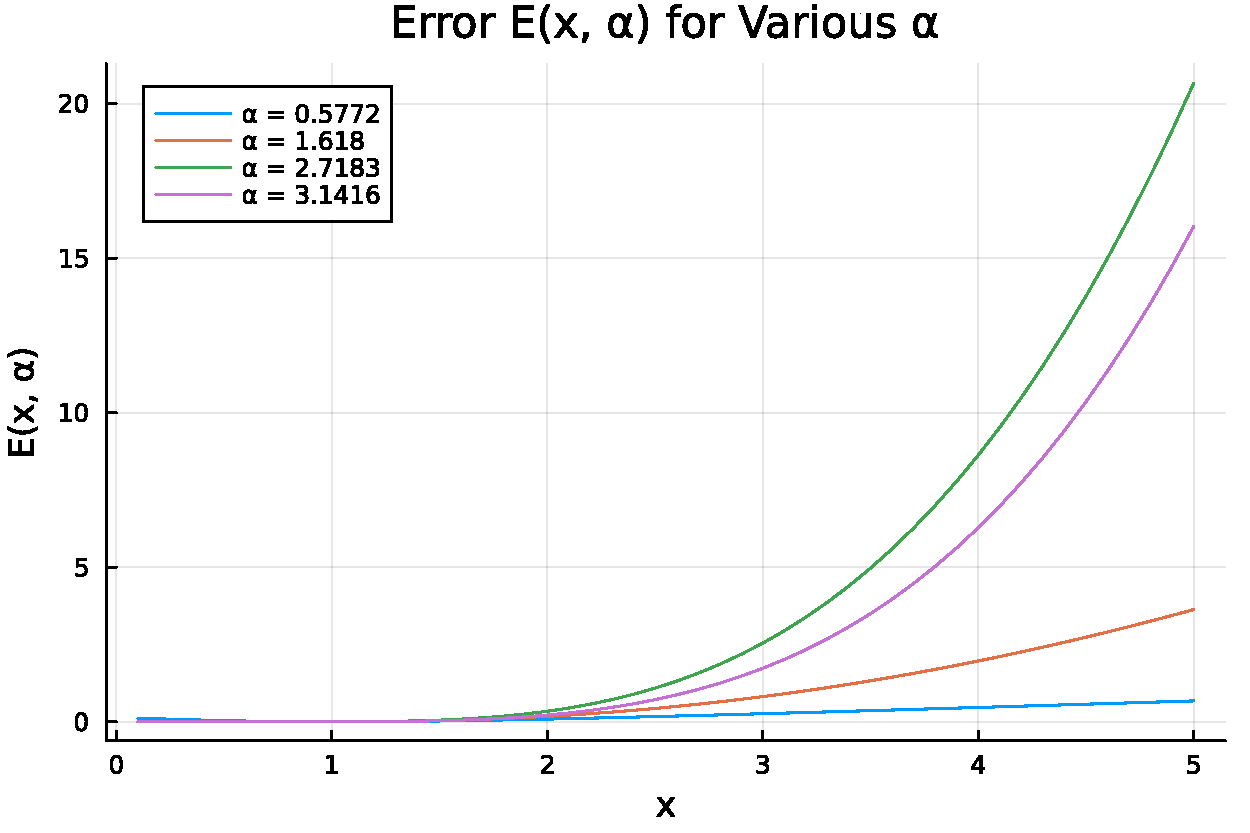
\includegraphics[width=0.8\textwidth]{figures/error_plot.pdf}
    \caption{Error of Caputo-Fabrizio MGF}
    \label{fig:error_MGF}
\end{figure}
It can be observed from the figure above that, in general for greater orders \(\alpha\), the error tends to increase. However, the greatest order of \(\alpha\) does not provide the greatest error. Instead it is the second greatest order of \(\alpha\) that does so. This may be explained by the fact that for values of \(\alpha\) in the middle of two integers, the value of \((1 - \beta)x + \beta\) will be the greatest. As a result, the fraction becomes small, so the error tends to increase.

This hypothesis is indeed confirmed in the following figure, which focuses on the growth rate of the error, for a fixed value of \(x\) and an increasing order \(\alpha\).

\begin{figure}[H]
    \centering
    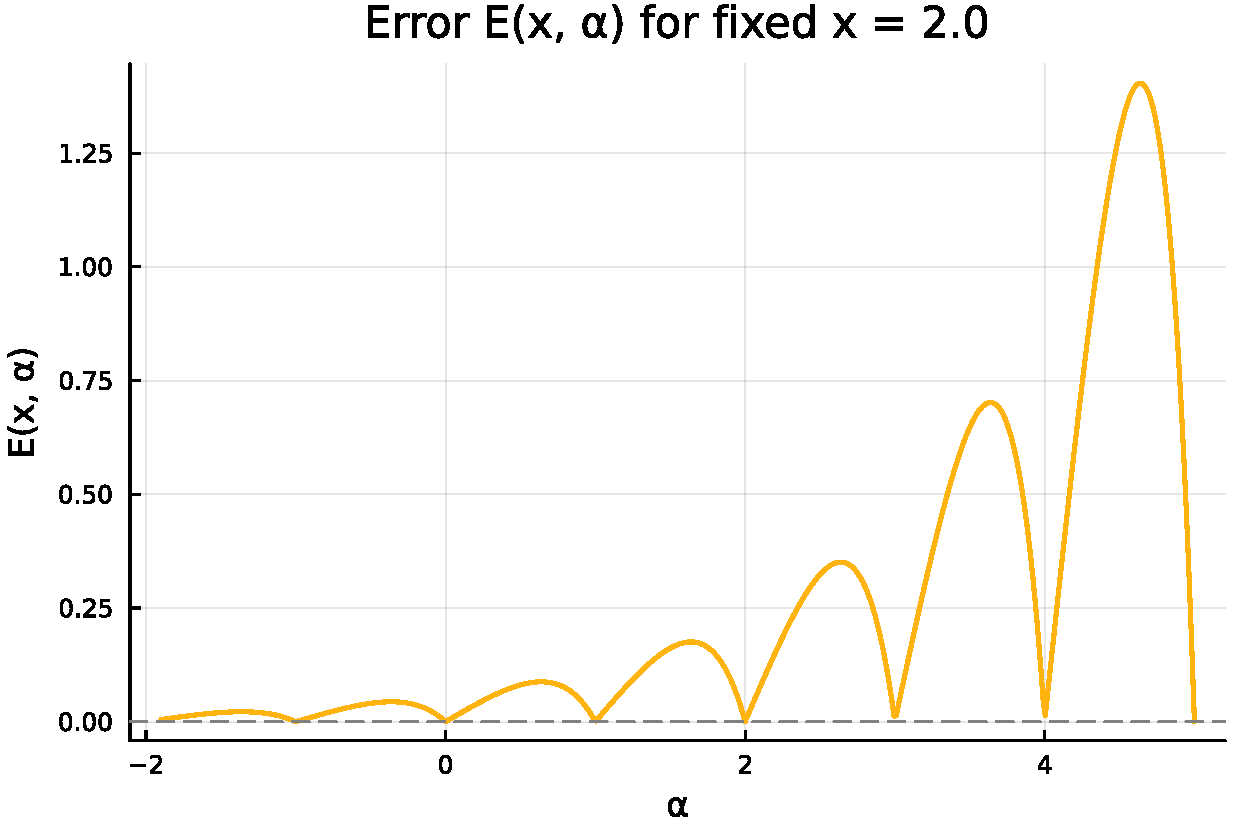
\includegraphics[width=0.8\textwidth]{figures/error_plot_fixed_x.pdf}
    \caption{Error of Caputo-Fabrizio MGF, for fixed x}
    \label{fig:error_MGF_fixed_x}
\end{figure}
Figure \ref{fig:error_MGF_fixed_x} indeed seems to indicate that for some \(\alpha \in (a, b)\), where \(a, b \in \mathbb{Z}\) consecutive integers that \(E(x, \alpha)\) attains it maximum value for some \(\alpha\) 'slightly greater' than \(\frac{a + b}{2}\). Figure \ref{fig:error_MGF_fixed_x} also reveals that the approximation error is considerably smaller for negative fractional moments compared to the positive ones. This suggests that, when negative moments are well-defined, the Caputo-Fabrizio MGF might still offer reasonable accuracy, despite its known limitations.

Note that within each integer interval, the function \(E(x, \alpha)\) appears to be concave. Thus, as is supported by figure \ref{fig:error_MGF_fixed_x}, it is only possible to obtain local maxima. Ideally, one would aim to analytically determine the optimal order \(\hat{\alpha}\) such that minimizes \(E(x, \hat{\alpha})\). However, due to the concavity of \(E(x, \hat{\alpha})\), such analyticcal minimization is not feasible. Figure \ref{fig:error_MGF_fixed_x} seems to suggest that order of \(\alpha\) near integer orders yields smaller approximation errors, which makes sensse intuitively. However, the latter is not rigorous evidence. Therefore, in the following section, we will analyse the numerical approximation errors of the Caputo-Fabrizio MGF by simulation. We will use numerical methods to try to obtain values \(\alpha\) which minimize the expression from theorem \ref{t: MGF_inaccurate}.





\section{Conclusion}\label{s:con}
The conclusion summarizes the results of your research.
Also it gives possible directions of further research.

\section*{Acknowledgements}
Place the acknowledgments section, if needed, after the main text, 
but before any appendices and the references. The section heading is not numbered.

\appendix

\section{(Appendix): Relevant functions and Identities}\label{s:appendices}
We define the (Euler-)Gamma function as follows:
\begin{definition}\label{d: eg}
    for \(\Re(z) > 0\), we have the following: \(\Gamma(z) = \int_{0}^{\infty} t^{z-1} e^{-t} dt\)
\end{definition}

The Gamma function can be seen as an extension of the factorial function, for non-integers. This function is defined for complex numbers and all there subsets (so also real numbers), as long as the condition above holds. For positive integers values \(z\), we have the following identity: \(\Gamma(z) = (z - 1)!\)
Other important identities, not necessarily for \(z\) an integer, are: 
\begin{itemize}
    \item \(\Gamma(z + 1) = z \Gamma(z)\)
    \item \(\Gamma(2) = \Gamma(1) = 1\)
    \item \(\Gamma(\frac{1}{2}) = \sqrt{\pi}\)
\end{itemize}

\begin{definition}\label{d: ff}
    The falling factorial is defined as follows: \((x)_n = \prod_{k = 0}^{n - 1} (x - k)\), which is a polynomial
\end{definition}
\begin{definition}
    For \(0 \leq k \leq n\), the Binomial Coefficient is defined as follows: \(\binom{n}{k}\), where \(n, k \in \mathbb{N}\).
\end{definition}
We can derive the following factorial identity, which is convenient to work with analytically: \(\binom{n}{k} = \frac{n!}{k! (n - k)!}\).
For numerically computing expressions containing the Binomial Coefficient, the following identity is computationally more efficient: \(\binom{n}{k} = \frac{(n)_k}{k!}\). With \((n)_k\) as in \ref{d: ff}.
Since we have established in \ref{d: eg} that \(\Gamma(z) = (z - 1)!\), we can rewrite our factorial identify to:
\[\binom{n}{k} = \frac{\Gamma(n + 1)}{\Gamma(k + 1) \cdot \Gamma( n - k  + 1)} = \frac{n}{k} \cdot\frac{\Gamma(n)}{\Gamma(k) \cdot \Gamma(n - k + 1)}\]

\begin{definition}\label{d: binomial}
    The binomial series is a generalization of the binomial formula, namely:
    \[(1 + x)^\alpha = \sum_{k = 0}^{\infty}\binom{\alpha}{k} x^k\]
\end{definition}

\begin{definition}
    Vandermonde's identity: for non-negative integers, \(k, l, m, n\), we have that \[\sum_{k = 0}^{l} \binom{m}{k} \cdot \binom{n}{l - k} = \binom{m + n}{l}\]
\end{definition}
A modification on the latter identity has been called the Chu-Vandermonde identity. This is the same identity, but it his been proven that the identities still hold for complex values \(m, n\) as long as \(l\) is a positive integer (\cite{askey75}).

For the interchange-ability of derivatives and integrals and sums, we can apply the following two theorems:

\begin{theorem}
    Leibnitz's Rule:
    Let \(f(x, \theta), a(\theta), b(\theta)\) be differentiable with respect to \(\theta\), then we have that:
    \[ \frac{d}{d\theta} \int_{a(\theta)}^{b(\theta)} f(x, \theta) dx = f(b(\theta), \theta) \frac{d b(\theta)}{d\theta} - f(a(\theta), \theta) \frac{d a(\theta)}{d\theta} + \int_{a(\theta)}^{b(\theta)} \frac{\partial f(x, \theta) }{\partial \theta} dx.\] For the special case, where \(a(\theta), b(\theta)\) are constant we have that: 
    \[\frac{d}{d\theta} \int_{a}^{b} f(x, \theta) dx =  \int_{a}^{b} \frac{ \partial f(x, \theta)}{ \partial d\theta}.\]
\end{theorem}

For the interchange-ability of derivatives and summations, the following theorem has been given by \cite{casella2002}:
\begin{theorem}
    Suppose that the series \(\sum_{x = 0}^{\infty} h(\theta, x)\) converges for all \(\theta\) in an interval \((a, b)\) of real numbers and 
    
    \begin{enumerate}[(i)]
        \item \(\frac{\partial h(\theta, x)}{\partial \theta}\) is continuous for all \(x\)
        \item \(\sum_{x = 0}^{\infty} \frac{\partial h(\theta, x)}{\partial \theta}\) converges uniformly on every closed bounded subinterval of \((a, b)\)
    \end{enumerate}
    Then:
    \[
    \frac{d}{d \theta} \left( \sum_{x = 0}^{\infty} h(\theta, x) \right) = \sum_{x = 0}^{\infty} \frac{\partial h(\theta, x)}{\partial \theta}
    \]
    
   
\end{theorem}


\newpage
\section{(Appendix): Proofs}\label{s:app_B}

\subsection{Proofs section \ref{s:calculus}}

\begin{proof}
    Proof of \ref{p: calculus}
    \begin{enumerate}[(i)]
        \item We will proof for the Riemann-Liouville derivative, the proof for the Caputo-Fabrizio derivative is very similar and the Grünwald-Letnikov derivative is a direct consequence of the linearity of the sum.
        \[ D^{\alpha} (a f(x) + b g(x)) = \frac{d^n}{dx^n}\frac{1}{\Gamma(n - \alpha)} \int_{0}^{x} (x - t)^{n - \alpha - 1} (a f(t) + b g(t)) dt \]
     
        \[= \frac{d^n}{dx^n}\left(\frac{a}{\Gamma(n - \alpha)} \int_{0}^{x} (x - t)^{n - \alpha - 1}  f(t)dt + \frac{b}{\Gamma(n - \alpha)} \int_{0}^{x} (x - t)^{n - \alpha - 1} g(t)dt\right) \] Where we simply split the integral and put the constants in front.
        \[= \frac{d^n}{dx^n}\frac{a}{\Gamma(n - \alpha)} \int_{0}^{x} (x - t)^{n - \alpha - 1}  f(t)dt + \frac{d^n}{dx^n} \frac{b}{\Gamma(n - \alpha)} \int_{0}^{x} (x - t)^{n - \alpha - 1} g(t)dt \] As the regular derivative operator is linear.
        \[ = a D^{\alpha} f(x) + b D^{\alpha} g(x) \]
        \item Intuitively, this makes perfect sense, as the 0-th derivative is just no derivative, so just the function \(f(x)\). But for these derivatives, a little bit more effort is required to prove this rather obvious fact.
        \newline 
        For the Grünwald-Letnikov derivative we get: \[D^0 f(x) = \lim_{h \to 0} \frac{1}{h^0} \sum_{k=0}^\infty (-1)^k \binom{0}{k} f(x - k h)
        = \lim_{h \to 0} \frac{1}{1} \sum_{k=0}^\infty (-1)^k \frac{0!}{k!(0- k)!} f(x - k h).\] The factorial identity of the binomial coefficient only holds for \(0 \leq k \leq \alpha\). Since \(\alpha = 0\) and k is always a positive integer lesser or equal to \(\alpha, k = 0\). Thus, we get:
        \[ = \lim_{h \to 0} \sum_{k=0}^\infty (-1)^0 \frac{0!}{0!(0- 0)!} f(x - 0 h) = \lim_{h \to 0} f(x - 0 h) = f(x).\]
        \newline
        For the Caputo-Fabrizio derivative, we obtain the following:
        \[ D^{0} f(x) = \frac{1}{1 - 0}  \int_{0}^{x} \exp\left(\frac{0}{1 -0}(x-t)\right) f'(t) dt = \int_{0}^{x}f'(t) dt = f(x).\]
        \newline
        Finally, for the Riemann-Liouville derivative, we can simply make use of \autoref{d: differintegral} and \autoref{r: integer} to note that in this context \(\alpha = 0\) is included in the natural integers. So \(D^\alpha = \frac{d^\alpha}{dx^\alpha} f(x) = {d^0}{dx^0} f(x) = f(x)\) by the first fundamental theorem of calculus.

        \item The proof for the Riemann-Liouville derivative is given by \cite{koning15}. And the proof for the Caputo-Fabrizio derivative is given by \cite{losada15}.For the Grünwald-Letnikov derivative, we get:
        \[ D^\alpha(D^\beta f(x)) = \lim_{h \to 0} \frac{1}{h^\alpha} \sum_{k=0}^\infty (-1)^k \binom{\alpha}{k}(  \frac{1}{h^\beta} \sum_{l=0}^\infty (-1)^l \binom{\beta}{l} f(x - l h - kh))\]
        \[= \lim_{h \to 0} \frac{1}{h^{\alpha + \beta}} \sum_{k=0}^\infty (-1)^k \binom{\alpha}{k} \sum_{l=0}^\infty (-1)^l \binom{\beta}{l} f(x - (k + l)h).\] We substitute \(m = k + l\) to deal with the dubble sums: 
        \[ \lim_{h \to 0} \frac{1}{h^{\alpha + \beta}} \sum_{m=0}^\infty f(x - mh)  \sum_{k=0}^m (-1)^k (-1)^{ m - k} \binom{\alpha}{k} \binom{\beta}{m - k}\] Now we make use of an identify from \autoref{s:appendices} to obtain:
        \[ = \lim_{h \to 0} \frac{1}{h^{\alpha + \beta}} \sum_{m=0}^\infty (-1)^m \binom{\alpha + \beta}{m} f(x - mh) = D^{\alpha + \beta} f(x).\]
        It can be shown in an exactly similar way that the latter expression is equal to \(D^\beta(D^\alpha f(x))\).

        
    \end{enumerate}
\end{proof}

\subsection{Proofs section \ref{s: moments}}

\begin{proof}
    Proof of proposition \ref{p: moments_1}
     
    \begin{enumerate}[(i)]
        \item If \(X\) is a discrete random variable, we get: \[\mathbb{E}[X^n] = \sum_{i} x_i^n f_X(x_i) = \infty, \mathbb{E}[X^k] = \sum_{i} x_i^k f_X(x_i)\]
        \[ = \sum_{i} x_i^n \cdot x^{k - n} f_X(x_i) \geq \sum_{i} x_i^n f_X(x_i) = \infty, \text{ as } k \geq n\]
        We can prove this for continuous random variables in a similar manner.
        \item This simply follows from the previous proposition, as the current proposition is just the contrapositive statement of the previous proposition.
    \end{enumerate}
\end{proof}

\begin{proof}
    Proof of Proposition \ref{p: moments}
    \begin{enumerate}[(i)]
        \item This is trivial. For \(X\) a continuous random variable, we get: 
        \[ M_X^{(0)}(t) = \int_{-\infty}^{\infty} x^0 e^{t x } f_X(x) dx = \int_{-\infty}^{\infty} 1 e^{0 x } f_X(x) dx = \int_{-\infty}^{\infty} f_X(x) dx.\] Assuming that \(f(x)\) is a PDF, this integrates to 1 by definition. If this integral is not equal to 1, this implies that \(f(x)\) is not a PDF. The proof for the discrete case is the same but with a summation instead of an integral sign.
        \item \[M_{\mu + \sigma X}(t) = \mathbb{E}[e^{(\mu + \sigma X)t}] = \mathbb{E}[e^{\mu t} \cdot e^{\sigma X t}].\] Since this is the expectation of \(x\), every term that is not dependent on \(x\) can be taken out of the summation:
        \[ = e^{\mu t} \cdot \mathbb{E}[e^{\sigma X t}] = e^{\mu t} \cdot M_{ X}(\sigma t)\]
        \item 
        \[M_{X+Y}(t) = \mathbb{E}[e^{(X + Y)t}] = \int_{-\infty}^{\infty} \int_{-\infty}^{\infty} e^{(x + y)t} f_{X, Y}(x, y) dx dy\] 
        \[= \int_{-\infty}^{\infty} \int_{-\infty}^{\infty} e^{xt} \cdot e^{yt} f_{X, Y}(x, y) dx dy.\] 
        \(f_{X, Y}(x, y)\) is the joint pdf for \(X, Y\). But we know that the latter is equal to \(f_X(x) \cdot f_Y(y)\), if \(X, Y\) are independent. Thus we get:
        \[ = \left(\int_{-\infty}^{\infty}  e^{xt} f_X(x) dx\right) \left(\int_{-\infty}^{\infty}  e^{yt} f_Y(y) dy\right) = M_X(t) \cdot M_Y(t).\] 
    \end{enumerate}
\end{proof}

\begin{proof}
    Proof of Theorem \ref{t: negative}:
Suppose for the moment that \( X \) is a positive random variable. Since \( x \cdot f_X(x) \) is integrable for \( x > 0 \), we have:

\[
    \mathbb{E}(X) = \int_0^\infty x \, dF(x) = \int_0^\infty \int_0^\infty e^{tx} \, dt \, dF(x).
\]

We can interchange the order of integration as follows:

\[
    \mathbb{E}(X) = \int_0^\infty e^{tx} \, dF(x) \, dt = \int_0^\infty M_X(-t) \, dt.
\]

The interchange of the order of integration is subject to \( \mathbb{E}(e^{-tX}) \) being integrable from \( t = 0 \) to \( t = \infty \).

Finally, by substituting \( X^{-1} \) for \( X \), we find:

\[
    \mathbb{E}(X^{-1}) = \int_0^\infty M_X^{-1}(-t) \, dt.
\]

There are two natural ways to generalize (1) to \( \mathbb{E}(X^{-1}) \); one way gives:

\[
    \mathbb{E}(X^{-n}) = \int_0^\infty \int_0^\infty \cdots \int_0^\infty M_X(-t_n) \, dt_n \cdots dt_2 dt_1, \tag{2}
\]

while the second way gives:

\[
    \mathbb{E}(X^{-n}) = \frac{1}{\Gamma(n)} \int_0^\infty t^{n-1} M_X(-t) \, dt.
\]
\cite{cressie1981}
\end{proof}

\begin{proof}
    Proof Theorem \ref{t: MGF_accurate}
    We consider \(X\) to be a continuous variable. The three MGF expressions are accurate if \(\mathbb{E}[X^\alpha] - M_X^{(\alpha)}(0) = 0\), in other words, if 
    \[\int_{-\infty}^{\infty} (x^\alpha - D^\alpha e^{tx}) \cdot f_X(x) dx = 0 \iff x^\alpha = D^\alpha e^{tx}\]
    where \(D^\alpha\) the differential operator of order \(\alpha\). Note that we are of course taking derivatives w.r.t. \(t\), not \(x\). The proof will be shown for the Grünwald-left derivative.
    \begin{enumerate}[(i)]
        \item \[\leftindex_{GL}{M}_X^{(\alpha)} = D^\alpha_{GL}(e^{tx})  = \lim_{h \to 0} \frac{1}{h^\alpha} \sum_{k=0}^\infty (-1)^k \binom{\alpha}{k} \exp(x(t - kh))\]
        \[= \exp(xt) \lim_{h \to 0} \frac{1}{h^\alpha} \sum_{k=0}^\infty (-1)^k \binom{\alpha}{k} \exp(-xh)^k\]
        \[= \exp(xt) \lim_{h \to 0} \frac{1}{h^\alpha} (1 - \exp(-xh))^\alpha\]
        (where we used the binomial series identity defined in \ref{d: binomial}). Now we use the Taylor expansion of \(\exp(-xh) = 1 - xh + \frac{(xh)^2}{2!} - \frac{(xh)^3}{3!} + ... - ...\). Since \(h \to 0\), we get: \(\exp(-xh) = 1 - xh + \mathcal{O}(h^2)\) (the rest of the terms are negligible).
        Thus we get:
        \[ \exp(xt) \lim_{h \to 0} \frac{1}{h^\alpha} (1 -(1 - xh + \mathcal{O}(n)))^\alpha = \exp(xt) \lim_{h \to 0} \frac{1}{h^\alpha} (h(x + \mathcal{O}(h)))^\alpha \]
        \[ = \exp(xt) \lim_{h \to 0} \frac{1}{h^\alpha} (h^\alpha((x + \mathcal{O}(h)))^\alpha) = \exp(xt) \lim_{h \to 0} (x + \mathcal{O}(h))^\alpha\]
        \[ = \exp(xt) x^\alpha.\]
        Finally, we take a value of \(t\) around 0 and obtain \(\leftindex_{GL}{M}_X^{(\alpha)}(0) = x^\alpha\) 
        \item We consider the Riemann-Liouville derivative: 
        \[D_{RL}^\alpha(e^{tx}) = \frac{d^n}{dt^n} \frac{1}{\Gamma(n -\alpha)}  \int_{-\infty}^{t} (t-s)^{n - \alpha-1} e^{sx} ds\]
        \cite{koning15} has shown that this derivative is equal to \(x^\alpha e^{tx}\). Thus, if we take a value of \(t\) around 0, we get: \(\leftindex_{RL}{M}_X^{(\alpha)}(0) = x^\alpha\)
    \end{enumerate}

    The proof also holds for the case when \(X\) is a discrete random variable.
\end{proof}

\begin{proof}
    Proof of Theorem \ref{t: MGF_inaccurate}
    We compute \[\leftindex_{CF}{M}_X^{(\alpha)} = D^\alpha_{CF}(e^{tx}) = \frac{d^n}{dt^n}\frac{1}{1 - \beta}  \int_{-\infty}^{t} \exp\left(\frac{-\beta}{1 - \beta}(t - s)\right) x \exp(xs) ds\]
    \[= \frac{d^n}{dt^n}\frac{x}{1 - \beta} \exp\left(\frac{-\beta t}{1 - \beta}\right) \int_{-\infty}^{t} \exp(s\left(\frac{\beta }{1 - \beta} + x \right)) ds  \text{ where } \beta = \alpha - n \text{ and } n = \lfloor \alpha \rfloor.\]
    Now let \(u = \frac{\beta}{1 - \beta} + x\), so we get:
    \[\frac{d^n}{dt^n}\frac{x}{1 - \beta} \exp\left(\frac{-\beta t}{1 - \beta}\right) \int_{-\infty}^{t} \exp(us) ds = \frac{d^n}{dt^n}\frac{x}{1 - \beta} \exp\left(\frac{-\beta t}{1 - \beta}\right) \frac{1}{u} exp(us)\Big|_{-\infty}^{t}\]
    \[= \frac{x}{1 - \beta} \exp\left(\frac{-\beta t}{1 - \beta}\right) \cdot \frac{1}{u} \cdot \exp(u t) = \frac{x \exp(xt)}{(1 - \beta)x + \beta}\]
    Now we apply the derivative of the above expression, with respect to \(t\), \(n\) times:
    \[\frac{d^n}{d t^n} \frac{x \exp(xt)}{(1 - \beta)x + \beta} = \frac{x^{n+1} \exp(xt)}{(1 - \beta)x + \beta}\]
    Now we take a value of \(t\) around 0 and obtain:
    \[\leftindex_{CF}{M}_X^{(\alpha)} = D^\alpha_{CF}(e^{tx}) = \frac{x^{n+1} }{(1 - \beta)x + \beta}.\]
    The latter expression is not equal to \(x^\alpha\), thus the error of \(\leftindex_{CF}{M}_X^{(\alpha)}\) is:
    \[x^\alpha - \frac{x^{n+1} }{(1 - \beta)x + \beta}\]

    
\end{proof}

\newpage

\section{Appendix C }\label{s: app_C}
\renewcommand{\arraystretch}{1.5}
\begin{longtable}{|p{2.5cm}|p{5.5cm}|p{4.5cm}|p{3.0cm}|}
\hline
\textbf{Distribution} & \textbf{PDF / PMF} & \textbf{MGF \(M_X(t)\)} & \textbf{Restrictions} \\
\hline
\endfirsthead
\hline
\textbf{Name} & \textbf{PDF / PMF} & \textbf{MGF \(M_X(t)\)} & \textbf{Restrictions} \\
\hline
\endhead

\( \text{Bernoulli}(p) \) & \( f(x) = p^x(1-p)^{1-x} \) & \( M_X(t) = (1 - p) + pe^t \) & \( 0 \leq p \leq 1, \ x \in \{0,1\}\) \\
\hline

\( \text{Binomial}(n, p) \) & \[ f(x) = \binom{n}{x} p^x (1-p)^{n-x} \] & \( M_X(t) = (1 - p + pe^t)^n \) & \( n \in \mathbb{N},\ 0 \leq p \leq 1 \) \\
\hline

Discrete Uniform  & \( f(x) = \frac{1}{N} \) & \( M_X(t) = \frac{1}{N} \sum_{k=1}^N e^{tk} \) & \( N \in \mathbb{N} \) \\
\hline

\( \text{Geometric}(p) \) & \( f(x) = p(1-p)^{x-1}\) & \( \frac{pe^t}{1 - (1 - p)e^t},\ t < -\ln(1 - p) \) & \( 0 < p \leq 1,\ x \geq 1  \) \\
\hline

\( \text{Poisson}(\lambda) \) & \[ f(x) = \frac{\lambda^x e^{-\lambda}}{x!}\] & \( \exp(\lambda(e^t - 1)) \) & \( \lambda > 0,\ x \geq 0  \) \\
\hline

\( \text{Beta}(\alpha, \beta) \) & \[ f(x) = \frac{1}{B(\alpha, \beta)} x^{\alpha-1}(1-x)^{\beta-1}\] & Messy & \( \alpha, \beta > 0,\ x \in (0,1)  \) \\
\hline

\( \text{Chi-Squared}(p) \) & \[ f(x) = \frac{1}{2^{p/2}\Gamma(p/2)} x^{p/2 - 1} e^{-x/2}\] & \( (1 - 2t)^{-p/2},\ t < 1/2 \) & \( p > 0,\ x > 0  \) \\
\hline

\( \text{Laplace}(\mu, \sigma) \) & \[ f(x) = \frac{1}{2\sigma} e^{-\frac{|x - \mu|}{\sigma}} \] & \( \frac{e^{\mu t}}{1 - (\sigma t)^2},\ |t| < \frac{1}{\sigma} \) & \( \sigma > 0 \) \\
\hline

\( \text{Exponential}(\beta) \) & \( f(x) = \frac{1}{\beta} e^{-x/\beta} \) & \( \frac{1}{1 - \beta t},\ t < 1/\beta \) & \( \beta > 0,\ x > 0 \) \\
\hline

\( \text{Gamma}(\alpha, \beta) \) & \[ f(x) = \frac{1}{\Gamma(\alpha)\beta^\alpha} x^{\alpha-1} e^{-x/\beta} \] & \( (1 - \beta t)^{-\alpha},\ t < 1/\beta \) & \( \alpha, \beta > 0,\ x > 0 \) \\
\hline

\( \text{Logistic}(\mu, \beta) \) & \[ f(x) = \frac{e^{-(x - \mu)/\beta}}{\beta(1 + e^{-(x - \mu)/\beta})^2} \] & \(e^{\mu t}\Gamma(1 - \beta t) \Gamma(1 + \beta t) \)& \( \beta > 0 \) \\
\hline

Normal \( \mathcal{N}(\mu, \sigma^2) \) & \[ f(x) = \frac{1}{\sqrt{2\pi \sigma^2}} e^{-\frac{(x - \mu)^2}{2\sigma^2}} \] & \( \exp\left( \mu t + \frac{\sigma^2 t^2}{2} \right) \) & \( \sigma > 0 \) \\
\hline

\( \text{Uniform}(a, b) \) & \( f(x) = \frac{1}{b - a}\) & \( \frac{e^{tb} - e^{ta}}{t(b - a)} \), \( t \neq 0 \) & \( a < b,\ x \in [a,b]  \) \\
\hline
\end{longtable}\label{t: MGF_Appendix}
\section{Appendix}\label{s:app1}
Place any appendices after the acknowledgments, starting on a new page.
The appendices are numbered
\textbf{A}, \textbf{B}, \textbf{C}, and so forth.
The appendices contain material that you would like to share with the
reader but that would hinder the flow of reading. For instance long
proofs of theorems, code of algorithms, data, etc.


%\printbibliography
% or in case of classic bibtex:
\bibliographystyle{chicago}
\bibliography{bib/bibfile}

\end{document}
